% Exemplo de relatório técnico do IC
% Criado por P.J.de Rezende antes do Alvorecer da História.
% Modificado em 97-06-15 e 01-02-26 por J.Stolfi.
% Last edited on 2003-06-07 21:12:18 by stolfi
% modificado em 1o. de outubro de 2008
% modificado em 2012-09-25 para ajustar o pacote UTF8. Contribuicao de
%   Rogerio Cardoso

\documentclass[11pt,twoside]{article}
\usepackage{techrep-PFG-ic}

%%% SE USAR INGLÊS, TROQUE AS ATIVAÇÕES DOS DOIS COMANDOS A SEGUIR:
\usepackage[brazil]{babel}
%% \usepackage[english]{babel}

%%% SE USAR CODIFICAÇÃO LATIN1, TROQUE AS ATIVAÇÕES DOS DOIS COMANDOS A
%%% SEGUIR:
%% \usepackage[latin1]{inputenc}
\usepackage[utf8]{inputenc}
\usepackage{graphicx}
\usepackage{listings}

\begin{document}

%%% PÁGINA DE CAPA %%%%%%%%%%%%%%%%%%%%%%%%%%%%%%%%%%%%%%%%%%%%%%%
% 
% Número do relatório
\TRNumber{01}

% DATA DE PUBLICAÇÃO (PARA A CAPA)
%
\TRYear{18}  % Dois dígitos apenas
\TRMonth{12} % Numérico, 01-12

% LISTA DE AUTORES PARA CAPA (sem afiliações).
\TRAuthor{G. L. da Silva \and E. Borin}

% TÍTULO PARA A CAPA (use \\ para forçar quebras de linha).
\TRTitle{Plataforma de processamento de dados sísmicos como serviço em Nuvem}

\TRMakeCover

%%%%%%%%%%%%%%%%%%%%%%%%%%%%%%%%%%%%%%%%%%%%%%%%%%%%%%%%%%%%%%%%%%%%%%
% O que segue é apenas uma sugestão - sinta-se à vontade para
% usar seu formato predileto, desde que as margens tenham pelo
% menos 25mm nos quatro lados, e o tamanho do fonte seja pelo menos
% 11pt. Certifique-se também de que o título e lista de autores
% estão reproduzidos na íntegra na página 1, a primeira depois da
% página de capa.
%%%%%%%%%%%%%%%%%%%%%%%%%%%%%%%%%%%%%%%%%%%%%%%%%%%%%%%%%%%%%%%%%%%%%%

%%%%%%%%%%%%%%%%%%%%%%%%%%%%%%%%%%%%%%%%%%%%%%%%%%%%%%%%%%%%%%%%%%%%%%
% Nomes de autores ABREVIADOS e titulo ABREVIADO,
% para cabeçalhos em cada página.
%
\markboth{da Silva e Borin}{Processamento sísmico como serviço na nuvem}
\pagestyle{myheadings}

%%%%%%%%%%%%%%%%%%%%%%%%%%%%%%%%%%%%%%%%%%%%%%%%%%%%%%%%%%%%%%%%%%%%%%
% TÍTULO e NOMES DOS AUTORES, completos, para a página 1.
% Use "\\" para quebrar linhas, "\and" para separar autores.
%
\title{Plataforma de processamento de dados sísmicos como serviço em Nuvem}

\author{Guilherme Lucas da Silva \and Edson Borin}

\date{}

\maketitle

%%%%%%%%%%%%%%%%%%%%%%%%%%%%%%%%%%%%%%%%%%%%%%%%%%%%%%%%%%%%%%%%%%%%%%

\begin{abstract} 
  Este trabalho busca criar uma plataforma que facilita o 
  processamento de dados sísmicos na nuvem, sem exigir do usuário conhecimento técnico dos
  novos conceitos que a nuvem traz consigo. A partir disso, tenta trazer
  mais agilidade, custos mais baixos e maior flexibilidade para os 
  engenheiros e desenvolvedores que trabalham em aplicações que 
  necessitam de alto poder computacional.

  Desta forma, o projeto foi iniciado com o objetivo de criar uma plataforma
  \emph{open source}, simples e replicável para qualquer 
  usuário. Os resultados foram muito positivos, alcançando o intuito de criar
  a plataforma somente com componentes \emph{open source} e replicável em
  diversas situações.
\end{abstract}

\section{Introducão}

Computação em Nuvem é um conceito que está cada vez mais presente no cotidiano de muitas pessoas. Mesmo sem perceber, uma grande quantidade de aplicações que usamos hoje 
em dia lançam mão desse conceito tão central para o desenvolvimento econômico e tecnológico de nossa sociedade contemporânea. Ele se baseia na capacidade de usarmos o
poder computacional de serviços como máquinas virtuais, bancos de dados e redes virtuais sem que o usuário tenha máquinas físicas com tais serviços 
instalados e configurados. Segundo o artigo intitulado Cloud Computing Security: A
Systematic Literature Review~\cite{UPP}, computação em nuvem é um modelo de rede que torna possível o acesso sob demanda de recursos computacionais configuráveis.
Entre as modalidades principais de serviços de computação em nuvem, temos três categorias:

\begin{itemize}

  \item \textbf{IaaS(\emph{Infrastructure as a Service}):} essa é a categoria que dá mais responsabilidade ao usuário. Essa exige que o desenvolvedor gerencie de maneira integral máquinas virtualizadas, 
  instale programas necessários, defina configurações e etc. Exemplo disso são máquinas virtuais que rodam sistemas operacionais GNU/Linux e são acessadas remotamente.
  \item \textbf{PaaS(\emph{Plataform as a Service}):} Aqui, o usuário não precisa se preocupar com pacotes de sistema, \emph{softwares} e configurações. Esse sabor de computação em nuvem, tenta 
  facilitar para que desenvolvedores consigam publicar suas aplicações. Isso significa que se, por exemplo, um usuário quiser expor uma aplicação, não é necessário
  instalar compiladores e pacotes necessários para rodar o programa naquela determinada linguagem.
  \item \textbf{SaaS(\emph{Software as a Service}):} essa é a modalidade que traz menos autonomia para o desenvolvedor, sendo que, através dela, todo o recurso é gerenciado pelo provedor de 
  nuvem que é consumido. Um exemplo que podemos citar para ilustrar são os bancos de dados como serviço, onde o usuário não se encarrega de nenhum tipo de infraestrutura, 
  somente usa o endereço que o provedor cede para o poder usufruir das possibilidades de armazenamento que a plataforma oferece.

\end{itemize}

Entre as vantagens de se adotar um modelo de computação em nuvem ao invés de investir em adquirir máquinas físicas, podemos citar:

\begin{itemize}
  \item \textbf{Custo:} devido à possibilidade de pagar somente pelo que está usando, ou seja, caso algum recurso esteja sendo pouco aproveitado, basta desligá-lo. Usuários desse tipo de 
  plataforma não gastarão para manter sistemas parados.
  \item \textbf{Escalabilidade:} A computação em nuvem permite que, caso a aplicação precise de mais poder computacional do que possui no momento, seja simples aumentar
  o número de instâncias ou o tamanho das máquinas, para atender mais usuários, gerando assim, mais receita.
  \item \textbf{Foco na aplicação:} desenvolvedores podem focar em escrever suas 
  aplicações, sem a preocupação de gerenciar infraestrutura e plataforma, o que pode ser trabalhoso.

\end{itemize}

Entre os principais provedores de nuvem pública atualmente temos a Microsoft Azure\footnote{Plataforma de computação em nuvem da Microsoft https://azure.microsoft.com/}, 
Amazon Web Services\footnote{Plataforma de computação em nuvem da Amazon https://aws.amazon.com/} e Google Cloud Platform\footnote{Plataforma de computação em nuvem do Google https://cloud.google.com/}, 
oferecendo opções diversas para computação em nuvem, desde máquinas virtuais até mesmo bancos de dados gerenciados.

Aplicações de alta performance computacional, ou HPC\footnote{do inglês \emph{High-Performance Computing}}, são uma gama de programas que necessitam de intenso poder computacional para 
completar seus objetivos. Entre essas tarefas, estão o processamento de dados sísmicos. Segundo K. Paladugu e S. Mukka~\cite{HPC}, supercomputação é usada para realizar operações matemáticas em alta velocidade. HPC é como supercomputação,
mas com o poder de processamento dos \emph{clusters}.
Ainda hoje, muitas dessas operações são feitas em servidores em institutos de pesquisas, por exemplo, podendo levar
a um custo excessivo, muito trabalho para gerenciamento de infraestrutura além de pouca agilidade e flexibilidade quanto à arquitetura. Assim, tais aplicações podem 
tirar muito proveito dos provedores de nuvem citados acima.

\section{Objetivos}
Esse trabalho tem como objetivo desenvolver uma plataforma \emph{open source} que torne simples para usuários que não conhecem conceitos de computação em nuvem 
executarem suas aplicações nesse tipo de ambiente. 
O desejado para o final da plataforma é que os usuários conseguissem processar 
os trabalhos sísmico sem necessariamente conhecer plataformas de nuvem.  
Ao final, é esperado a criação de uma plataforma \emph{web}, que tinha como principais funcionalidades:

\begin{itemize}
  \item \textbf{Submissão e gerenciamento de dados:} essa funcionalidade é a responsável pelo \emph{upload} de dados sísmicos que serão usados nos processamentos, além de consultar quais já foram submetidos, baixá-los e também
  excluí-los, caso necessário. 
  \item \textbf{Submissão e gerenciamento de binários:} esse componente do projeto é semelhante ao que detalhamos acima, porém, ao invés dos dados sísmicos, os artefatos que são gerenciados são os 
  binários das aplicações que serão utilizados nos processos.
  \item \textbf{Definição de tarefas sísmicas:} utilizando os dados e binários submetidos a partir das duas funcionalidades citadas anteriormente, o objetivo é conseguir lançar um processamento que combina os dados e 
  binários, além dos argumentos necessários.
  \item \textbf{Obtenção dos resultados:} ao final dos processos, é desejado que se consiga obter todos os seus resultados de maneira simples e rápida.
\end{itemize}

\section{Relevância}
Ao buscar por outras soluções que têm o mesmo intuito da plataforma que esse trabalho tem por objetivo desenvolver, notamos a sua relevância, uma que vez que é difícil achar outros programas \emph{open source} que executam tal tarefa.
Além da unicidade que o trabalho possui no cenários atual, ele se torna relevante já que ele pode abstrair os novos conceitos e a curva de aprendizado que vem junto com a computação em nuvem. Assim é possível
tirar proveito de todos os benefícios que foram citados acima, levando a possibilidade de um uso mais inteligente dos recursos, baixando custos e aumentando a produtividade.

\section{Arquitetura do Sistema}
Para o sucesso do projeto, ao começo dele, foi decidido que faríamos uma plataforma \emph{web}. Essa decisão  foi tomada devido à facilidade de desenvolver para esse tipo de plataforma, além do alcance que 
plataformas \emph{web} possuem, já que é praticamente obrigatório nos dispositivos com acesso à internet (celulares e computadores) a existência de um
navegador instalado. Além disso, vale ressaltar que desde o início do projeto todo o código estava aberto no Github\footnote{Serviço para compartilhamento de código fonte www.github.com}, 
já que foi uma premissa desde o início do projeto que este seria \emph{open source}.

Ao iniciar a análise do problema, foi possível notar que uma arquitetura de nuvem que se encaixa nesse problema é a de \emph{Work Queues} (Filas de Trabalho), que segundo Brendan Burns em seu livro
Designing Distributed Systems, em um sistema de filas de trabalho existe uma trabalho em lote para ser executado. Cada parte do trabalho é independente do outro e pode ser executado sem nenhuma interação. 
~\cite{BB}.
Isso é o que foi buscado, uma vez que os trabalhos eram intensivos, demoravam um tempo significativo para serem reproduzidos e eram independentes um do outro. Assim, o que gostaríamos era que trabalhos fossem submetidos
a uma fila e, alguma unidade de computação o usasse para executar uma tarefa.

\begin{figure}[!h]
  \centering
  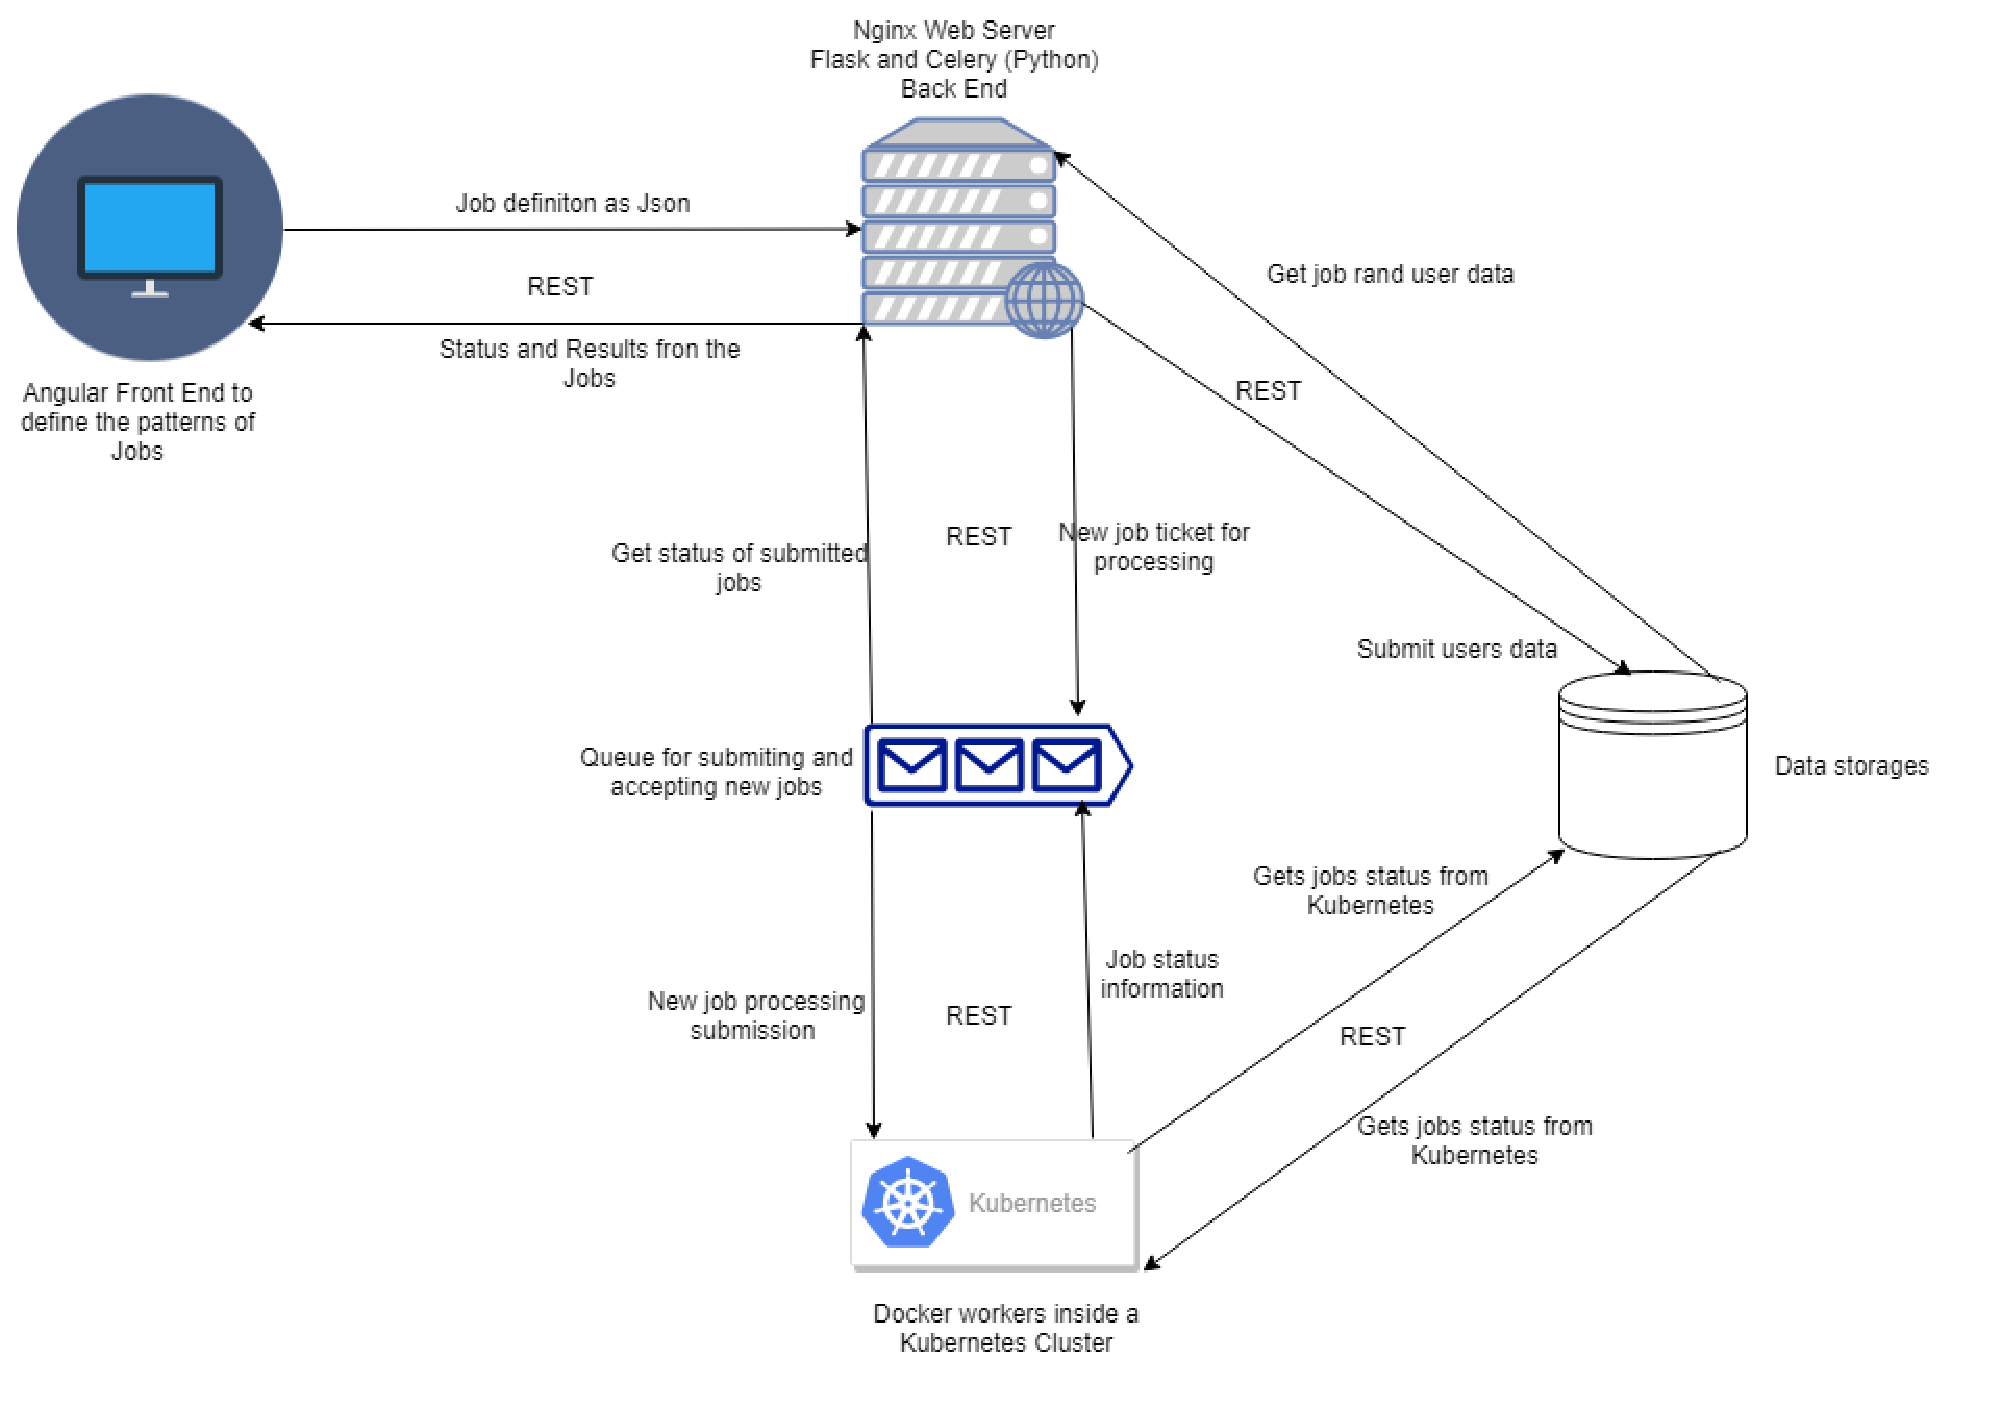
\includegraphics[scale=0.4]{arch.eps}
  \caption{Arquitetura inicial do projeto e exemplo de filas da trabalho distribuídas}
  \label{fig:archtec}
\end{figure}

A Figura~\ref{fig:archtec} ajuda a explicar como é o funcionamento dessa arquitetura e o desenho inicial do projeto.

A plataforma foi separada em duas grandes partes:

\begin{itemize}
  \item \textbf{\emph{Front End}:} a parte que o usuário realmente vê, o código que irá rodar no navegador do seu dispositivo. 
  \item \textbf{\emph{Back End}:} essa é a porção da plataforma responsável por características que são invisíveis ao usuário. Entre elas, podemos citar acesso à camada de armazenamento, autenticação,
  submissão de dados para a nuvem, etc.
\end{itemize}

Existem alguns componentes que foram usados em comum entre essas duas partes:

\begin{itemize}
  \item \textbf{Docker\footnote{Programa que realiza virtualização em nível de Sistema Operacional, também conhecido como conteinerização https://www.docker.com/}:} 
  uma maneira muito simples de empacotar as aplicações, isolando dependências, garantindo que o \emph{deploy} seja feito da maneira correta. Assim, é possível entregar as aplicações completas, com
  todos os requisitos necessários instalados, o que dá maior agilidade durante o ciclo de desenvolvimento.
  \item \textbf{Nginx\footnote{Servidor Web \emph{open source} https://www.nginx.com/}:} servidor \emph{web open source} escalável e fácil de configurar. Foi usado tanto para servir o \emph{back end} quanto o \emph{front end}. 
  A outra opção para esse trabalho seria o Apache Web Server, porém o Nginx se mostrou mais simples e rápido de ter aplicações rodando.
\end{itemize}

\subsection{\emph{Front End}}

Para o desenvolvimento do \emph{front end}, foram definidas de antemão como seria a composição geral das telas e o fluxo da aplicação. Assim, a visão geral das telas, foi definida da seguinte maneira:

\begin{figure}[!h]
  \centering
  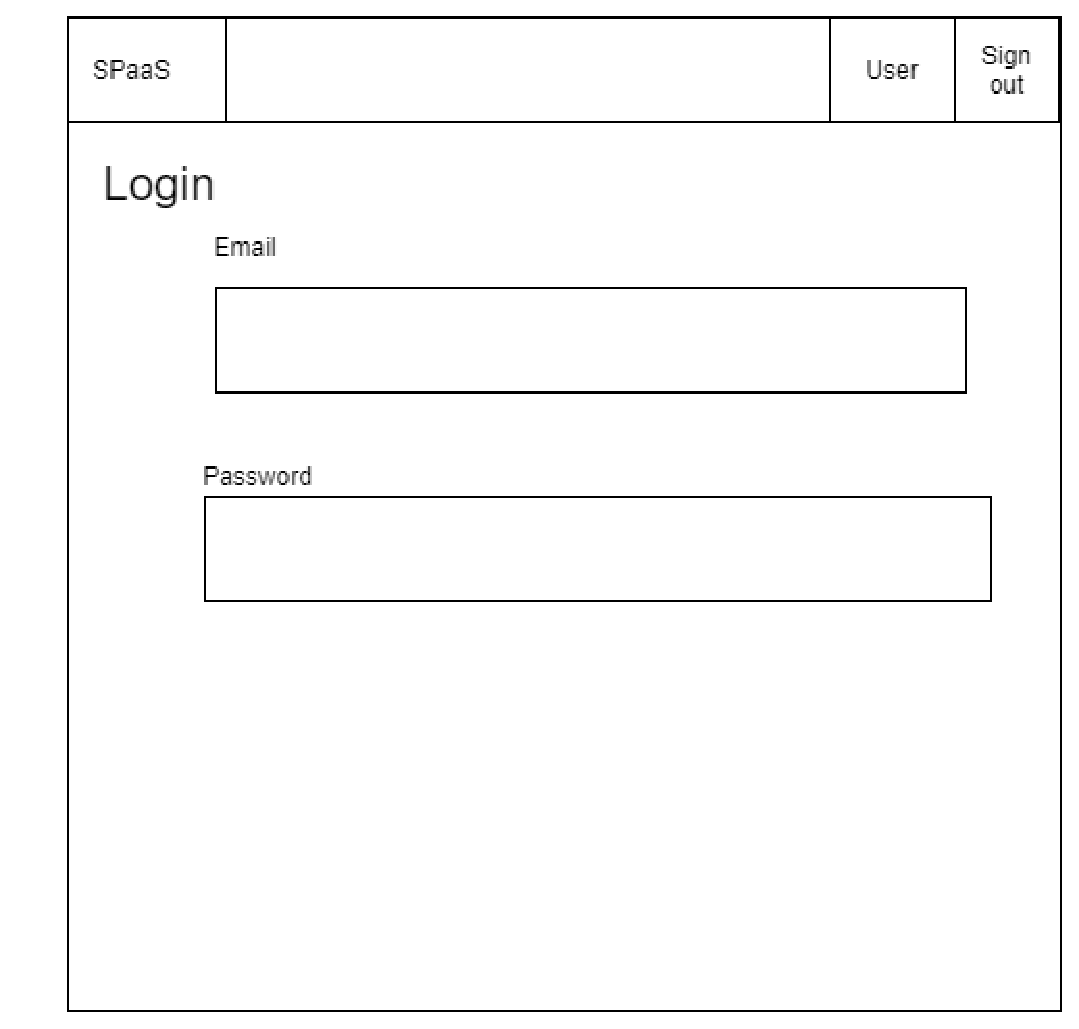
\includegraphics[scale=0.4]{login.eps}
  \caption{Tela de Login}
  \label{fig:loginScreen}
\end{figure}

A Figura~\ref{fig:loginScreen} mostra como definimos quais informações deveriam estar na tela para que o usuário pudesse se conectar a plataforma. Como mostrado, 
as informações necessárias para entrar no sistema eram \emph{e-mail} e senha que foram previamente cadastrados.

\begin{figure}[!h]
  \centering
  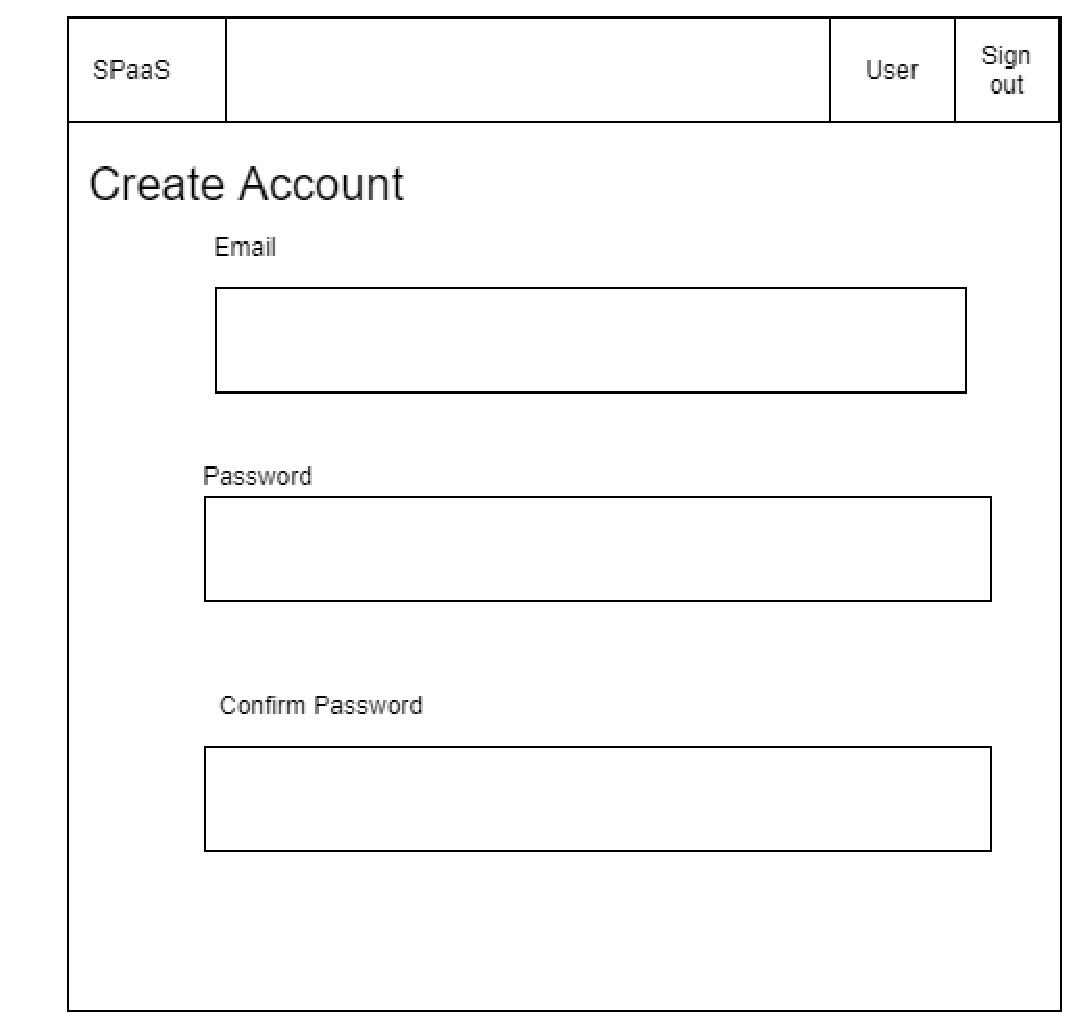
\includegraphics[scale=0.4]{account_reg.eps}
  \caption{Tela de criação de conta}
  \label{fig:createScreen}
\end{figure}

A Figura~\ref{fig:createScreen} deixa claro quais foram as informações que eram requeridas para se criar uma conta no sistema. 

\begin{figure}[!h]
  \centering
  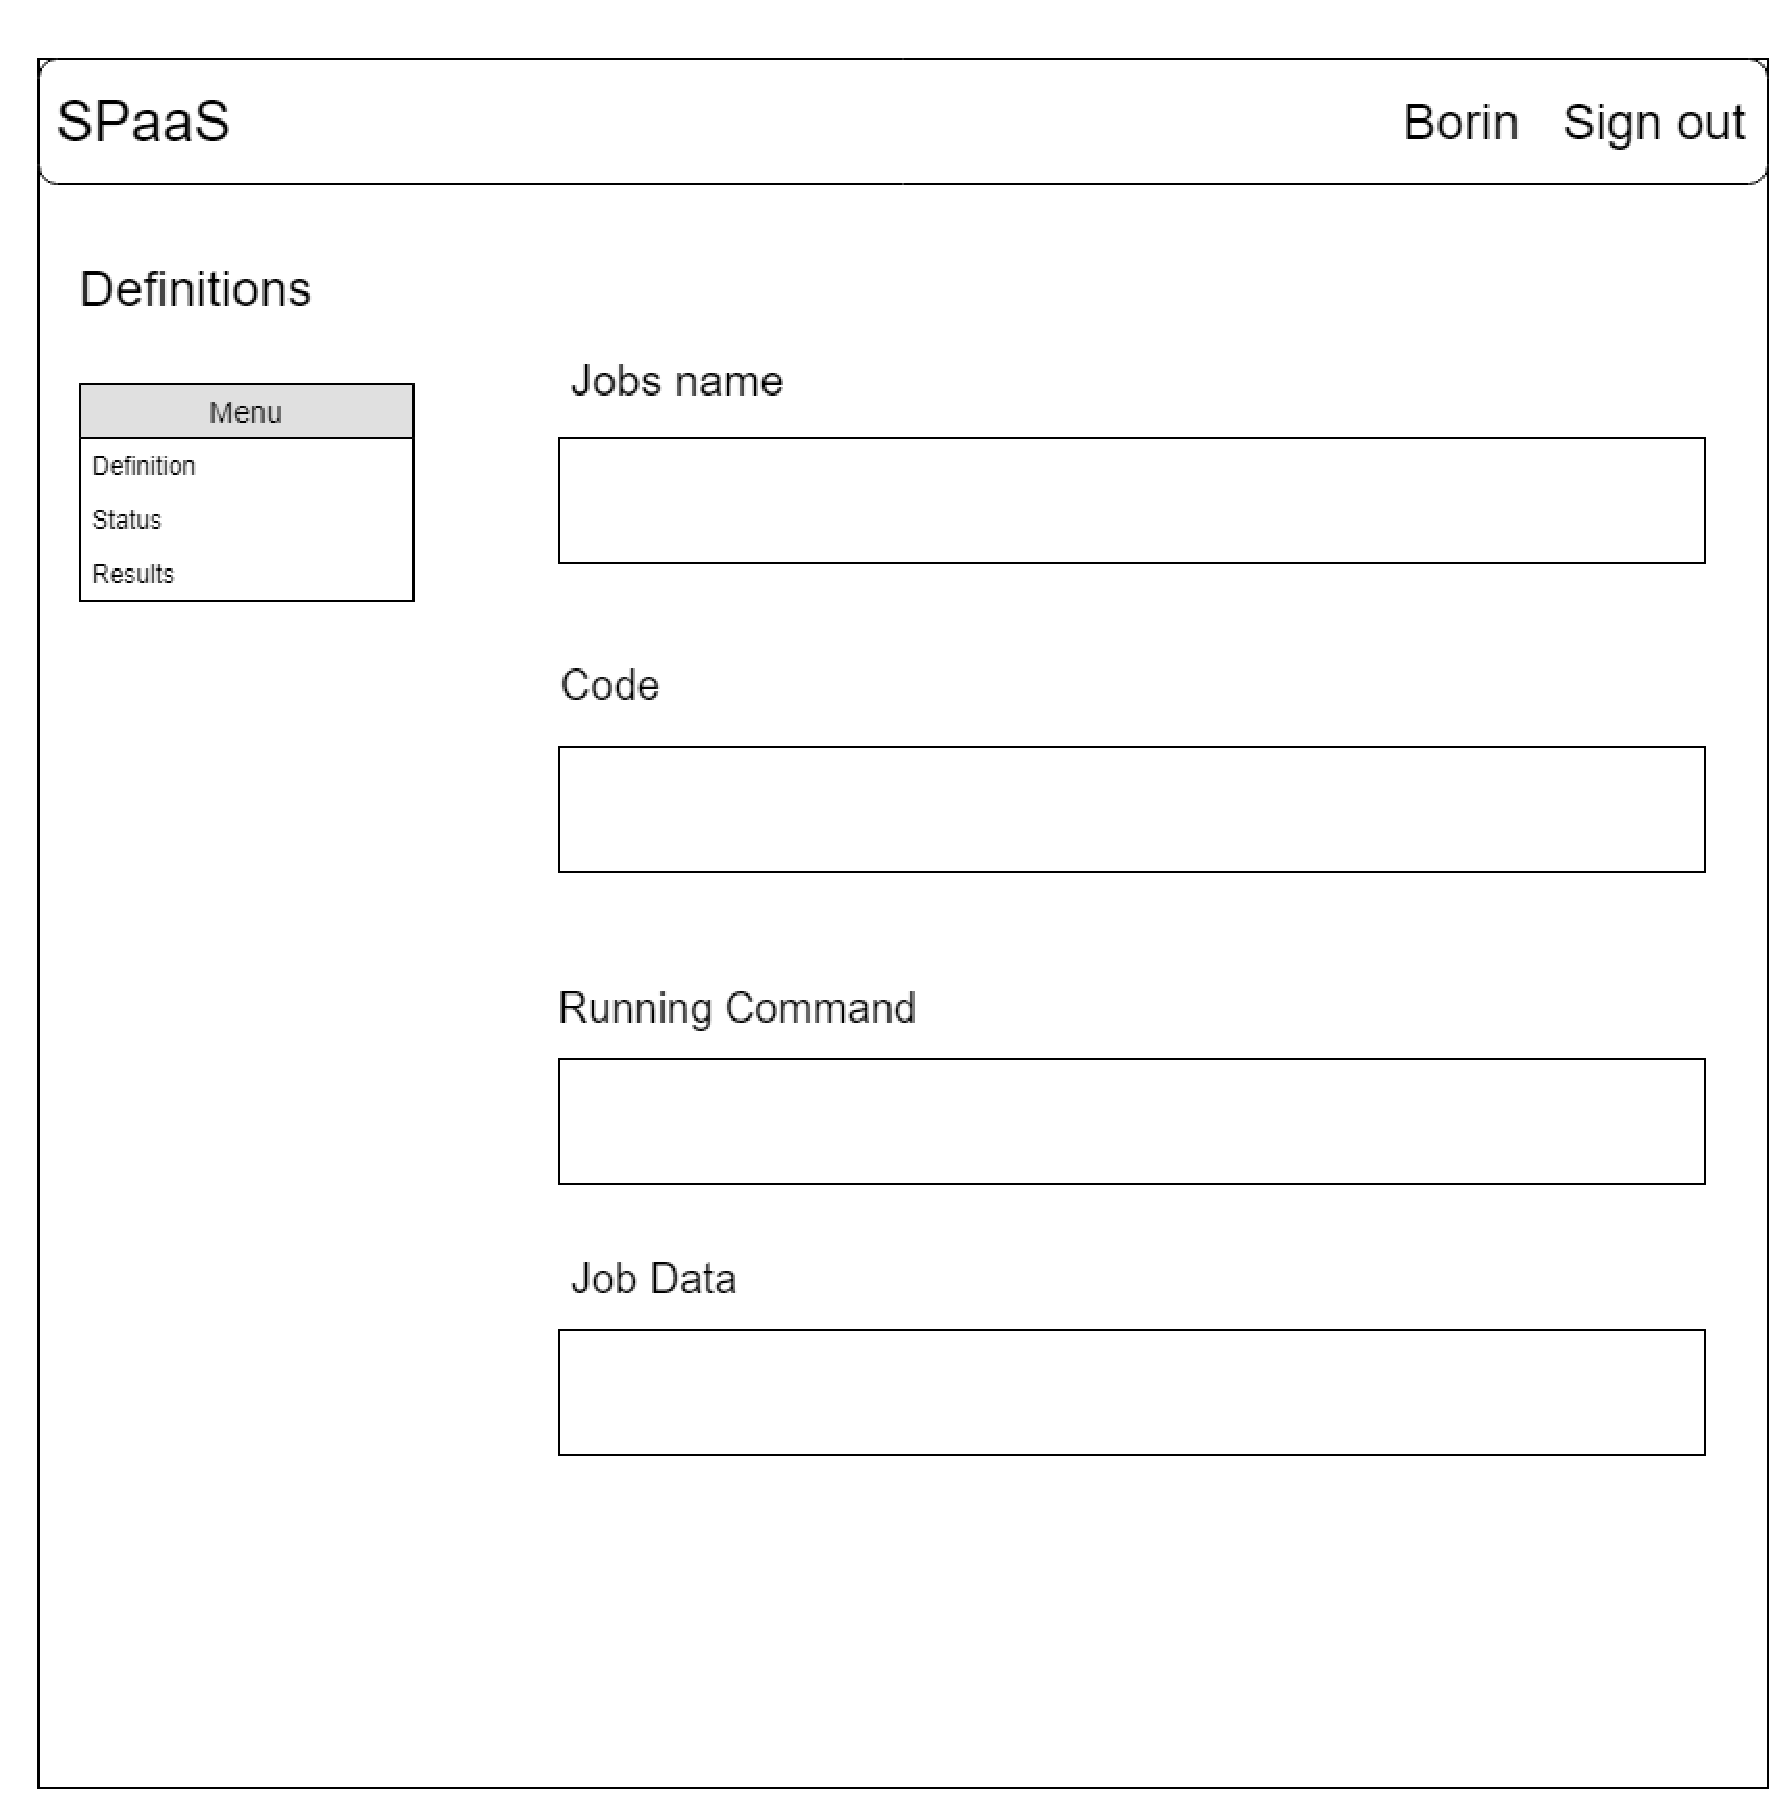
\includegraphics[scale=0.2]{First_screen.eps}
  \caption{Tela de definição dos trabalhos}
  \label{fig:definitionScreen}
\end{figure}

A Figura~\ref{fig:definitionScreen} exemplifica como imaginamos a tela de definição de um trabalho para ser executado. Nesse primeiro protótipo, foi pensado que somente 
as informações ilustradas na tela, eram o suficiente.

\begin{figure}[!h]
  \centering
  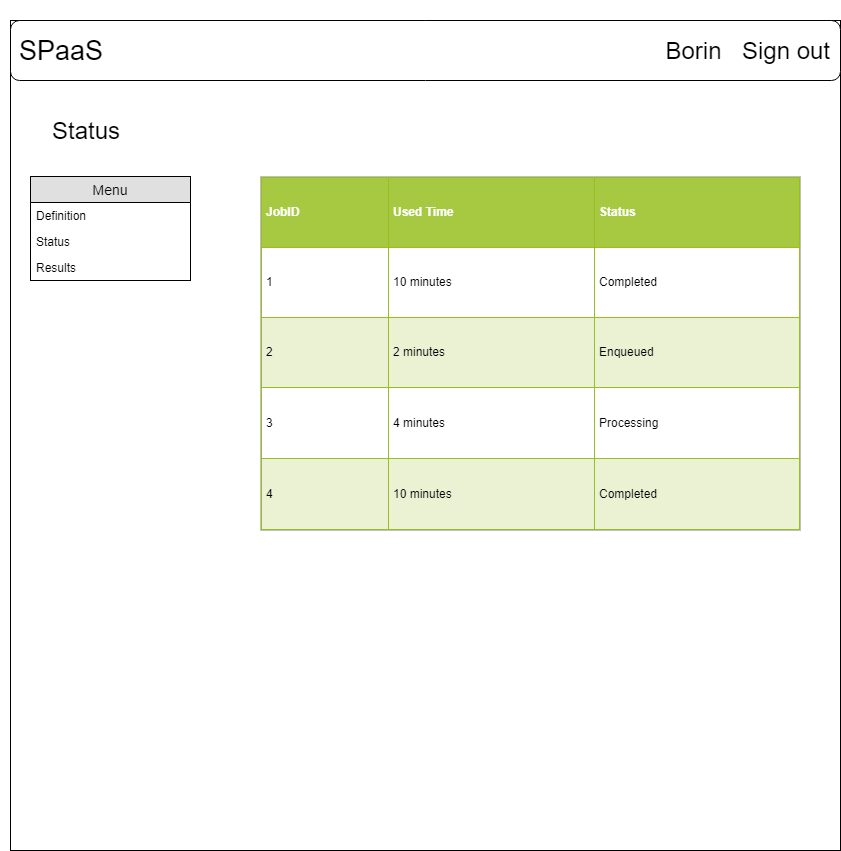
\includegraphics[scale=0.2]{Second_screen.eps}
  \caption{Tela de observação do status}
  \label{fig:statusScreen}
\end{figure}

\begin{figure}[!h]
  \centering
  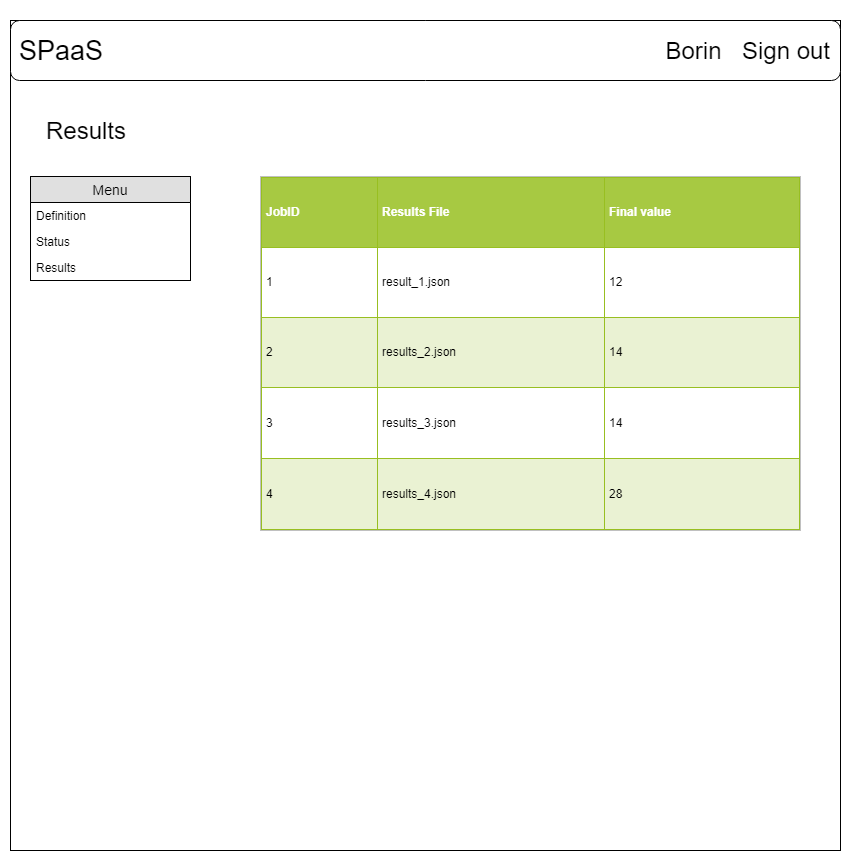
\includegraphics[scale=0.2]{Third_screen.eps}
  \caption{Tela de obtenção dos resultados}
  \label{fig:resultsScreen}
\end{figure}

O protótipo da tela de status dos trabalhos está ilustrada na Figura~\ref{fig:statusScreen}. Simples a princípio, uma tabela mostrando o status de cada trabalho. 

A Figura~\ref{fig:resultsScreen} mostra como foi pensada a obtenção dos resultados.

\begin{figure}[!h]
  \centering
  \includegraphics[scale=0.2]{tcc_flow.eps}
  \caption{Fluxo entre os componentes da plataforma}
  \label{fig:flowScreen}
\end{figure}

Vale ressaltar que essa ideia inicial foi pensada com poucas funcionalidades para a plataforma. Assim, o fluxo de todo o trabalho definitivo foi 
repensado para algo mais próximo do representado na Figura~\ref{fig:flowScreen}. Nesse fluxo definido, os quadrados representam as telas, com suas respectivas interações com 
as camadas de armazenamento que são necessárias para completar suas tarefas com sucesso. Assim, detalhando cada componente da solução:

\begin{itemize}
  \item \textbf{\emph{Data Management}:} componente responsável pelo gerenciamento dos dados sísmicos da plataforma. A intenção nesse componente é ser capaz de adicionar, remover e 
  movê-los de um tipo de armazenamento mais caro (porém mais rápido) para um mais barato, e mais lento. 
  \item \textbf{\emph{Flow Management}:} componente responsável por determinar uma sequência de passos que devem ser feitos para completar uma tarefa (\emph{tasks}). Diferente das tarefas,
  aqui a definição é de um conjunto de \emph{tasks}, encadeadas para a obtenção de um resultado maior.
  \item \textbf{\emph{Tools Management}:} essa funcionalidade procura realizar o gerenciamento dos binários que serão executados. Assim como o componente responsável pelo gerenciamento
  dos dados sísmicos, esse componente busca dar a possibilidade de adicionar, mover e excluir binários da plataforma.
  \item \textbf{\emph{Running Tasks}:} nessa tela, é desejado que o usuário consiga ver qual é o status dos processamentos que iniciou. Status como Executando e Pronto são alguns dos 
  possíveis.
  \item \textbf{\emph{New Tasks}:} responsável por definir novas tarefas a serem rodadas. Os atributos necessários para essa definição são binário, dado sísmico 
  e argumentos para a execução acontecer com sucesso. 
  \item \textbf{\emph{Results}:} os resultados dos processamentos executados estarão aqui, organizados pela processamento que o gerou.
\end{itemize}

\subsection{\emph{Front End}}

Como tecnologias para o desenvolvimento da nossa plataforma, especificamente para o \emph{front end}, foram escolhidas as seguintes tecnologias:

\begin{itemize}
  \item \textbf{Angular\footnote{\emph{Framework open source} para desenvolvimento \emph{web} https://angular.io/}:} \emph{framework} para desenvolvimento de aplicações \emph{web open source}, desenvolvido inicialmente pelo Google e agora também mantido pela comunidade. Usa como linguagem de desenvolvimento o
  Typescript\footnote{Linguagem criada pela Microsoft. https://www.typescriptlang.org/}. A escolha desse \emph{framework} aconteceu pois ele é bastante produtivo e completo, já encapsulando todo o conceito de serviços, estilo de página e 
  linguagem de marcação, roteamento, etc. Assim, com esse \emph{framework} ainda é necessário conhecer linguagens de marcação como HTML e CSS, mas a junção de todos esses conceitos fica mais simples.
  \item \textbf{Bootstrap\footnote{Conjunto de ferramentas \emph{open source} que ajuda na estilização de páginas https://getbootstrap.com/}:} \emph{framework} que possui o estilo de vários componentes \emph{web} prontos, como tabelas, menus laterais, barras superiores, etc. É o que muitos \emph{sites} usam hoje em dia, como é o caso do Github.
  Estilizar páginas \emph{web} pode se tornar um trabalho complicado e demorado, por isso optamos por usar um \emph{framework}.
\end{itemize}

Foi garantido que o \emph{deploy} fosse feito da maneira mais simples e flexível para o cliente. Então, foi usado o servidor \emph{web} Nginx para isso. Além disso, também foi disponibilizado um Dockerfile, que possibilita
o \emph{deploy} da solução de maneira simples e direta sobre contêineres Docker.

\subsection{\emph{Back End}}

Ao início do desenvolvimento do \emph{back end}, buscamos escolher quais seriam as melhores tecnologias para esse componente, além de definir como seriam as rotas e contratos que a API do \emph{back end} iria expor
para que o \emph{front end} pudesse consumir de forma eficaz e direta, garantindo assim, o desacoplamento entre os dois componentes. Assim, os componentes que escolhemos para o \emph{back end} foram os seguintes:

\begin{itemize}
  \item \textbf{Python\footnote{https://www.python.org/}:} linguagem criada por Guido Van Rossum, muito presente nos dias de hoje devido a sua extensa gama de aplicações, que vão desde embarcados até sistemas de análise de dados de alto 
  desempenho. A escolha dela foi devido principalmente a bibliotecas maduras para desenvolvimento de API's \emph{back end}, filas de trabalho distribuídas e conectores com bancos de dados.

  \item \textbf{Flask\footnote{\emph{Framework web open source} para Python http://flask.pocoo.org/}:} \emph{framework} para desenvolvimento de APIS para Python. Foi escolhido devido a agilidade para colocar uma API rodando. Além disso, é simples entender como a aplicação está funcionando,
  fator muito crítico para decidirmos a escolha desta, uma vez que o projeto tem como premissa ser \emph{open source}. Ao invés de Python/Flask, foram cogitadas também ASP.NET
  com C\# e NodeJS. A primeira foi descartada devido a complexidade para criarmos uma API. NodeJS não foi escolhido devido a dificuldade que novos programadores podem enfrentar para compreender as
  funcionalidades em um primeiro momento, quando necessitassem aumentar o projeto.

  \item \textbf{Celery\footnote{\emph{Framework open source} para tarefas distribuídas em Python http://www.celeryproject.org/}:} uma vez escolhido Python e Flask como ferramentas para o desenvolvimento da solução, foi natural a escolha do Celery como ferramenta para filas de trabalho. Existem
  casos de sucesso documentados por engenheiros e desenvolvedores que usaram essa combinação com eficácia. O Celery é um componente do Python que é o responsável por gerenciar, submeter e obter
  resultados de uma fila de trabalho, de uma maneira muito simples. Além disso, dá suporte a vários componentes de mensageria, como por exemplo, RabbitMQ\footnote{Plataforma \emph{open source} de Mensageria https://www.rabbitmq.com/}, 
  Redis, Amazon SQS\footnote{Sistema de mensageria da plataforma AWS https://aws.amazon.com/sqs/}.  

  \item \textbf{Redis\footnote{Armazenamento de dados em memória \emph{open source} https://redis.io/}:} após a escolha de qual biblioteca iríamos usar para facilitar a execução das filas de trabalho, que foi o Celery, foi preciso escolher o componente para a mensageria do projeto, ou seja, o
  componente que realmente é responsável por armazenar e distribuir as mensagens relacionadas aos trabalhos submetidos na solução. Entre as opções estavam RabbitMQ, Redis e Amazon SQS. Essas são as que melhor se 
  integravam com o Celery, sendo possível obter todas as suas funcionalidades com os três. Porém, Amazon SQS é uma opção dependente a um provedor de nuvem, o que complica o desenvolvimento do projeto, caso seja 
  preciso usar outra \emph{cloud} diferente da AWS. RabbitMQ e Redis ofereciam funcionalidades muito parecidas, porém o Redis foi escolhido, devido ã sua documentação e suas outras funcionalidades
  que podem ser aproveitadas também, como, por exemplo, \emph{cache} e armazenamento de dados em memória.

  \item \textbf{MongoDB\footnote{Banco de Dados NoSQL \emph{open source} https://www.mongodb.com/}:} para o armazenamento dos dados de cadastro de usuários, informações sobre argumentos de cada binário e etc., a escolha foi um banco de dados NoSQL, o MongoDB. A decisão deste
  foi natural, uma vez que os dados que estavam trafegando entre um serviço e outro tinham uma estrutura muito parecida com os documentos que são guardados nesse tipo de banco, não sendo necessário se preocupar
  em transformar os dados para os esquemas presentes em tabelas SQL.

  \item \textbf{Blob Storage\footnote{Armazenamento de caráter genérico no Microsoft Azure https://azure.microsoft.com/en-us/services/storage/blobs/}:} o Blob Storage da Microsoft Azure foi selecionado pois era necessário uma espécie de armazenamento de propósito geral. Aqui ele está sendo usado para armazenamento dos dados sísmicos e
  binários. Foi escolhido devido à integração que possui com Python. Outras opções existentes eram, por exemplo, Amazon S3 \footnote{Armazenamento genérico na AWS https://aws.amazon.com/pt/s3/}, que oferece serviços semelhantes. Outra opção era deixar esses dados 
  no disco de máquinas virtuais e compartilhá-los por meio de servidores, porém, isso aumentaria a complexidade e dificultaria a tarefa de gerenciar esse tipo de infraestrutura.
\end{itemize}

\subsection{Ferramentas para \emph{Deploy}}

Como dito anteriormente, ao iniciar o projeto, não era desejado que utilizássemos somente um modelo de \emph{deployment}. Assim, para facilitar o \emph{deploy} da aplicação independente
do modo que foi escolhido para isso, foi criado uma série de scripts em ferramentas específicas para ajudar. Existem dois modelos que estão sendo facilitados:

\begin{itemize}
  \item \textbf{Kubernetes\footnote{Orquestrador de containêres \emph{open source} https://kubernetes.io/}:} orquestrador de containêres famoso nos dias de hoje, que tem como principal funcionalidade tornar mais simples, escalável e performática o \emph{deploy}
  de aplicações baseadas em containêres. Nascida dentro do Google, a partir do Borg, que segundo o artigo publicado pelo Google~\cite{BORG}, é um gerenciador de \emph{cluster} que roda centenas de milhares de processamentos,
  de milhares de diferentes aplicações entre uma série de \emph{clusters},
  atualmente está sob a jurisdição da Cloud Native Computing Foundation\footnote{Cloud Native Computing Foundation https://www.cncf.io/} e é \emph{open source}. Foi uma
  das plataformas que foi visada por ter apresentado relevância nos últimos tempos, com todos os grandes provedores de nuvem oferecendo opções gerenciadas dessa 
  ferramenta.
  \item \textbf{Ansible\footnote{Gerenciador de configuração \emph{open source} https://www.ansible.com/}:} um modelo comum de deploy de aplicações é o baseado em máquinas virtuais. Nesse caso, é bom garantir que todas as dependências necessárias para que a 
  aplicação rode com sucesso estejam instaladas. Nesse aspecto, o Ansible se mostra extremamente eficaz. Essa ferramenta surgiu da Red Hat e também é mantida \emph{open source}, sendo um
  ótimo gerenciador de configurações, o que torna possível escrever configurações como código, garantindo que a aplicação sempre terá sucesso para ser executada.
\end{itemize}

\section{Resultados}

\subsection{Arquitetura}

\begin{figure}[!h]
  \centering
  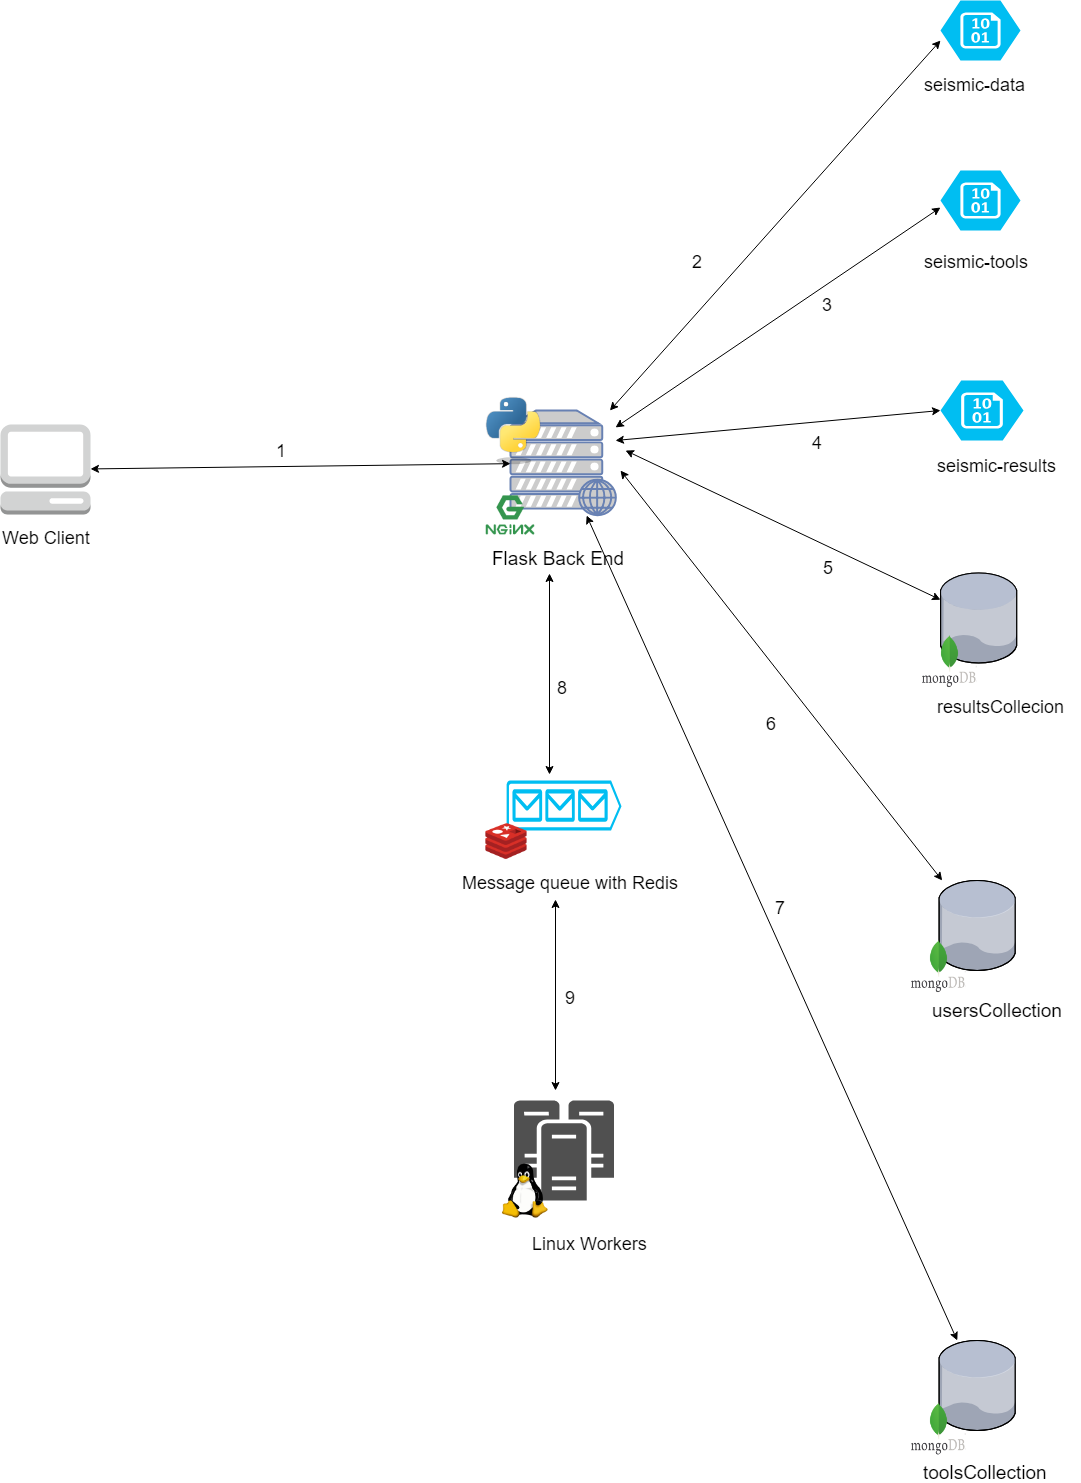
\includegraphics[scale=0.2]{final_arch.eps}
  \caption{Arquitetura final do projeto}
  \label{fig:finalArch}
\end{figure}

Após seguir todo o experimento citado acima, foi alcançado um resultado muito próximo do esperado. A arquitetura final do projeto, está ilustrada na Figura~\ref{fig:finalArch}.

Dada a arquitetura final do projeto mostra na Figura~\ref{fig:finalArch} os componentes mostrados têm, cada um, a seguinte função:

\begin{itemize}
  \item \textbf{\emph{Web Client}:} componente que é executado no lado do cliente. Seguimos com o que foi proposto no início do projeto e explicado durante o procedimento, ou seja, todo o código do lado do cliente 
  foi escrito em Typescript, com o auxílio do \emph{framework} Angular, a estilização das páginas foi feita com Bootstrap e servido via Nginx.
  \item \textbf{Flask \emph{Back End}:} responsável por receber todas as requisições que saem do \emph{front end}. Funciona como um \emph{gateway}. Também foi seguido o plano inicial de escrever todo o \emph{back end} com
  Python, Flask e Celery. Esse é o componente que possui mais responsabilidades: autenticação, comunicação com a fila com o auxílio do Celery, acesso aos Blobs e acesso ao banco.
  \item \textbf{Linux \emph{Workers}:} componente que é responsável pela execução propriamente dita dos pedidos de trabalho. Com o auxílio do Celery, esperam por pedidos entrarem na fila, e assim que isso acontece, os executam. 
  É possível ter um \emph{cluster} de máquinas com esse papel, aumentando o paralelismo das execuções.
  \item \textbf{\emph{Message queue with Redis}:} também parte do plano inicial, a fila de mensagens com o Redis foi a maneira mais eficaz e resiliente que encontramos de desacoplar o \emph{back end} dos Linux \emph{workers}. Assim
  O \emph{back end} submete uma mensagem com as definições para a execução de um trabalho na fila e algum \emph{worker} obteria essa requisição, realizando o processamento necessário. Aqui vale uma observação 
  importante: A escolha do Celery e do modelo de filas de trabalhos distribuídas, que já foi explicada anteriormente, torna possível, além de desacoplar o \emph{back end} dos \emph{workers}, a execução de
  processamentos em paralelo e distribuídos, não criando um gargalo na solução, possivelmente ocasionado pelo grande número de pedidos na fila.
  
  \begin{figure}[!h]
    \centering
    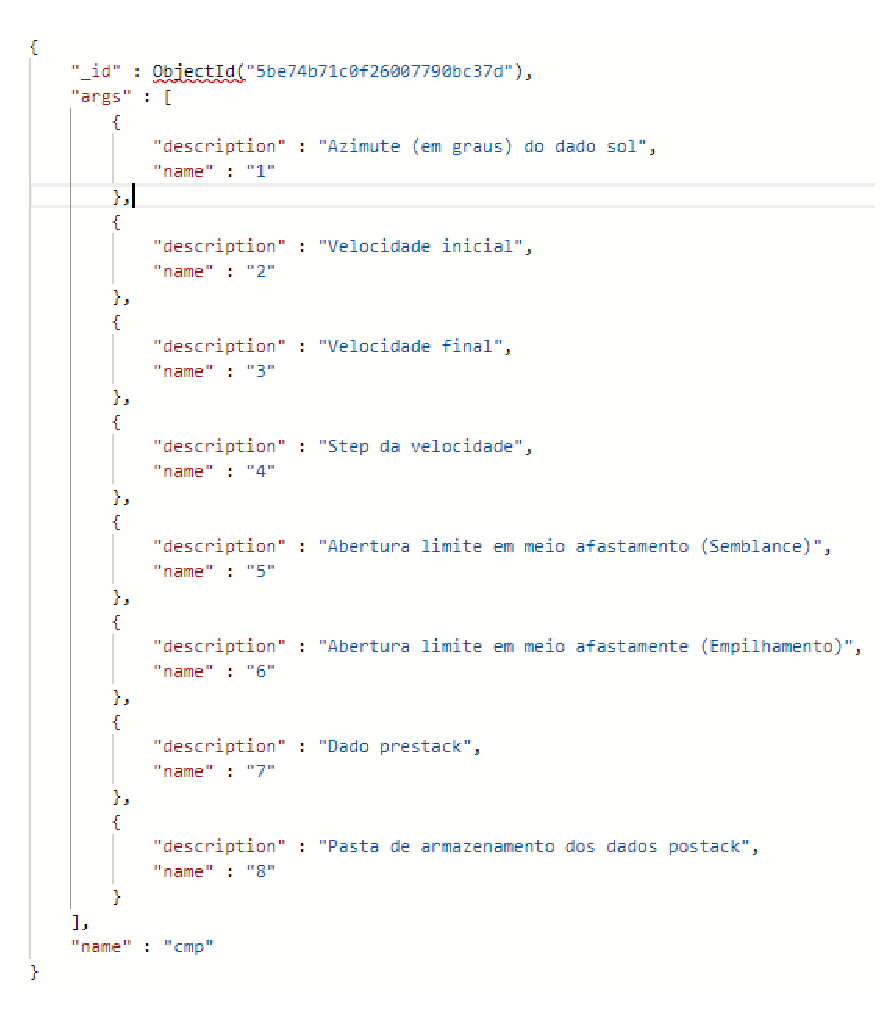
\includegraphics[scale=0.5]{tools_model.eps}
    \caption{Modelo presente na coleção de ferramentas binárias}
    \label{fig:toolsCollection}
  \end{figure}

  \item \textbf{toolsCollection:} coleção dentro do banco que guarda informações sobre os binários que estão armazenados. Novos dados são inseridos nela quando um novo binário é armazenado, quando
  um novo pedido de processamento será incluído e também quando um binário é excluído.
  O modelo que está sendo usado para guardar essas informações é o que está na Figura~\ref{fig:toolsCollection}
  
  \begin{figure}[!h]
    \centering
    
\includegraphics[scale=0.5]{results.eps}
    \caption{Modelo presente na coleção de resultados}
    \label{fig:resultsCollection}
  \end{figure}

  \item \textbf{resultsColleciton:} coleção de documentos no banco que armazena os dados dos resultados, armazena o id do processamento, dado e binário usado, além dos argumentos. 
  Essa coleção é acessada após o término de cada processamento, para salvar as informações do resultado e também para listar resultados. O modelo segue o padrão da Figura~\ref{fig:resultsCollection}.

  \begin{figure}[!h]
    \centering
    
\includegraphics[scale=0.5]{users_model.eps}
    \caption{Modelo presente da coleção de usuários}
    \label{fig:usersCollection}
  \end{figure}

  \item \textbf{usersCollection:} usada para armazenamento de dados dos usuários, como senha e \emph{e-mail} para autenticação. Um novo registro é criado nessa coleção quando um usuário cria uma nova conta. 
  A coleção também é acessada para autenticação de um novo usuário. Para que todos esses processos sejam executados com sucesso, o modelo usado é o da Figura~\ref{fig:usersCollection}.

  \item \textbf{seismic-tools:} Blob usado para armazenar os binários submetidos pelos usuário. Acessado pelo componente de gerenciamento de ferramentas quando uma nova é inserida na plataforma 
  e quando um novo processamento acontece.
  \item \textbf{seismic-data:} Blob que armazena os dados sísmicos submetidos. Também são acessados pelo componente de gerenciamento de dados quando um novo dado é incluído, excluído e na execução dos 
  trabalhos, já que é necessário baixar esses dados.
  \item \textbf{seismic-results:} outro Blob. Esse, responsável por armazenar os resultados dos processamentos. Todos os resultados são empacotados em um arquivo tar.gz\footnote{ utilitário de compressão de dados https://www.gzip.org/} e disponibilizados para \emph{download}, 
  no componente de resultados.
\end{itemize}

Vale notar aqui que, usamos somente uma instância de bancos de dados, com coleções diferentes para cada tipo de aplicação, as \emph{Collections}. Também usamos a mesma estratégia para o Blob. Foi usada somente 
uma conta de armazenamento no Microsoft Azure, com pastas separadas para cada uso, seismic-data, seismic-tools e seismic-results. 

\subsection{Rodando a aplicação}

Esta seção é dedicada à explicação de como executar cada componente da plataforma:

\subsubsection{\emph{Front End}}

Para rodar o \emph{front end}, todas as variáveis de ambiente estão no caminho front-end/src/environments. Nesse caminho existem dois arquivos, environment.ts e environment.prod.ts.
O primeiro contém os valores das variáveis de ambiente que serão consideradas durante o desenvolvimento, ou seja, quando o comando

\begin{lstlisting}[language=bash]
  $ ng serve 
\end{lstlisting}

é usado. Assim, a única variável que deve ser alterada é a apiUrl, que deve apontar para o \emph{back end}. Assim para compilar o projeto e servi-lo usando um servidor \emph{web}, os comandos que 
devem ser rodados são os seguintes: 

\begin{lstlisting}[language=bash]
  $ npm install 
  $ npm run build -- --output-path=./dist/out --configuration production
\end{lstlisting}

Isso gerará uma pasta ./dist/out que, quando colocadas no caminho /usr/share/nginx/html de um computador com nginx instalado, irá servir a aplicação do \emph{front end}.

Outra maneira de rodar o \emph{front end} é via Docker. Existe um Dockerfile dentro da pasta \emph{front end} que facilita o \emph{deploy}. Existem dois comandos que devem ser rodados nesse caso, um
para construir a imagem do Docker e outro para rodá-la:

\begin{lstlisting}[language=bash]
  $ docker build -t my-angular-project:prod .
  $ docker run -p 80:80 my-angular-project:prod
\end{lstlisting}

Ao acessar o \emph{localhost},a tela inicial do projeto será mostrada.

\subsubsection{\emph{Back End}}

Aqui, assim como no \emph{front end}, também existe a possibilidade de rodar o código nativamente ou dentro de um container Docker. Para executar o \emph{back end} nativamente, dentro da pasta \emph{back end}
existe o arquivo main.py e o requirements.txt. O arquivo de requirements.txt mostra quais são os pacotes necessários para rodar a aplicação. Também é preciso definir três
variáveis de ambiente, que são:

\begin{itemize}
  \item SPASS\_CONNECTION\_STRING: String de conexão do MongoDB.
  \item SPASS\_DATA\_BLOB\_KEY: Chave referente ao Blob que guardará todos os componentes citados anteriormente: resultados, dados e binários.
  \item SPASS\_CELERY\_BROKER: String de conexão do \emph{broker} do Celery, que, no caso do nosso experimento é o Redis.
\end{itemize}

Assim, após adicionar essas variáveis de ambiente, basta, dentro da pasta \emph{back end}, rodar os seguintes comandos:

\begin{lstlisting}[language=bash]
  $ pip3 install -r requirements.txt
  $ python3 main.py
\end{lstlisting}

Caso a opção seja por rodar o \emph{back end} com Docker, os comandos são:

\begin{lstlisting}[language=bash]
  $ docker build -t flask-back .
  $ docker run -p 5000:5000 -e SPASS\_CONNECTION\_STRING="<value>" -e SPASS\_DATA\_BLOB\_KEY="<value>" -e SPASS\_CELERY\_BROKER="<value>" flask-back
\end{lstlisting}

Nesse caso, o \emph{back end} estará escutando na porta 5000.

\subsubsection{Worker}

Para os \emph{workers}, dentro da pasta \emph{back end}, basta executar:

\begin{lstlisting}[language=bash]
  $ pip3 install -r requirements.txt
  $ celery worker -A main.celery -l info
\end{lstlisting}

Nos \emph{workers} também é necessário declarar as mesmas variáveis de ambiente do \emph{back end}, citadas anteriormente. 
Como a proposta é ter vários workers para executar as tarefas em paralelo, foi criado um \emph{playbook} Ansible, para configurar várias máquinas para 
executar essas tarefas. Para isso, com o Ansible instalado basta executar dentro da pasta devops:

\begin{lstlisting}[language=bash]
  $ ansible-playbook worker_config.yaml
\end{lstlisting}

\subsection{Telas finais}

Assim, após apresentar a arquitetura final, são apresentados os componentes, com suas respectivas telas. 

\begin{figure}[!h]
  \centering
  
\includegraphics[scale=0.3]{final_login.eps}
  \caption{Tela final do \emph{login}}
  \label{fig:finalLogin}
\end{figure}

Na tela final de \emph{login}, Figura~\ref{fig:finalLogin}, existem dois campos: \emph{e-mail} e senha. Além disso, caso você não possua uma conta, é possível criar no canto superior direito.

\begin{figure}[!h]
  \centering
  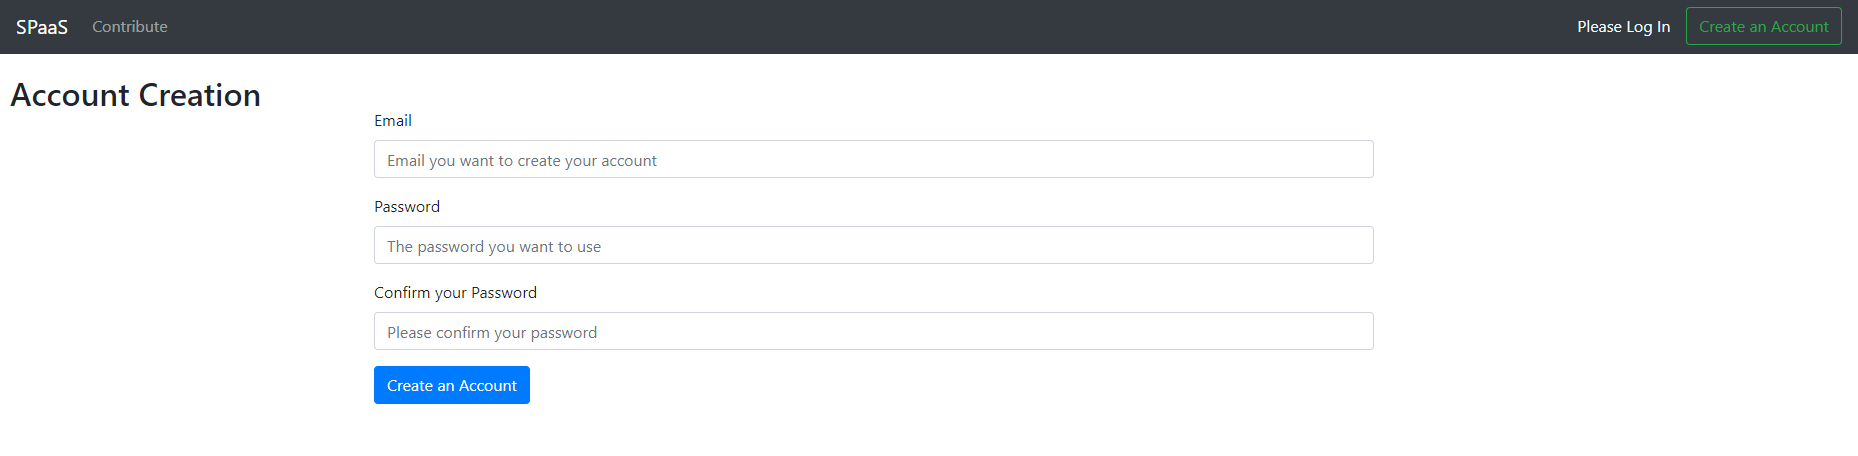
\includegraphics[scale=0.3]{final_create.eps}
  \caption{Tela final de criação de contas}
  \label{fig:finalCreate}
\end{figure}

 Ao escolher a opção de criar uma conta, o usuário será direcionado é a Figura~\ref{fig:finalCreate}, onde será possível criar uma nova conta com \emph{e-mail} e senha, que deve ser confirmada.

\begin{figure}[!h]
  \centering
  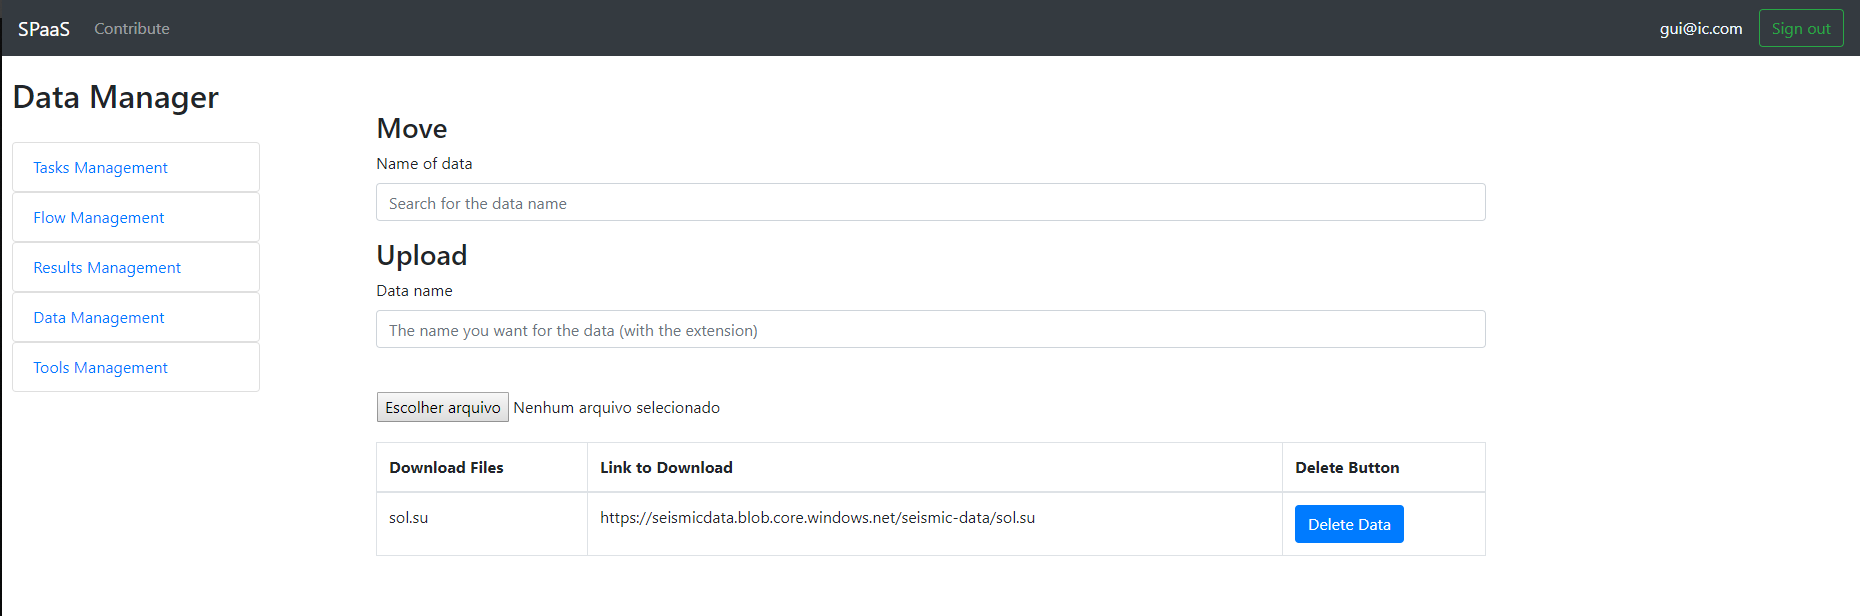
\includegraphics[scale=0.3]{data_final.eps}
  \caption{Tela final de gerenciamento de dados sísmicos}
  \label{fig:finalData}
\end{figure}

Na Figura~\ref{fig:finalData} é possível observar como todas as funcionalidades que foram planejadas no início estão sendo contempladas. Na seção de \emph{upload}, é possível definir um nome para o dado, e escolher o 
arquivo que será submetido. Além disso, a tabela abaixo mostra todos os dados que foram submetidos, com o \emph{link} para \emph{download} e também a opção de deletar os já existentes.

\begin{figure}[!h]
  \centering
  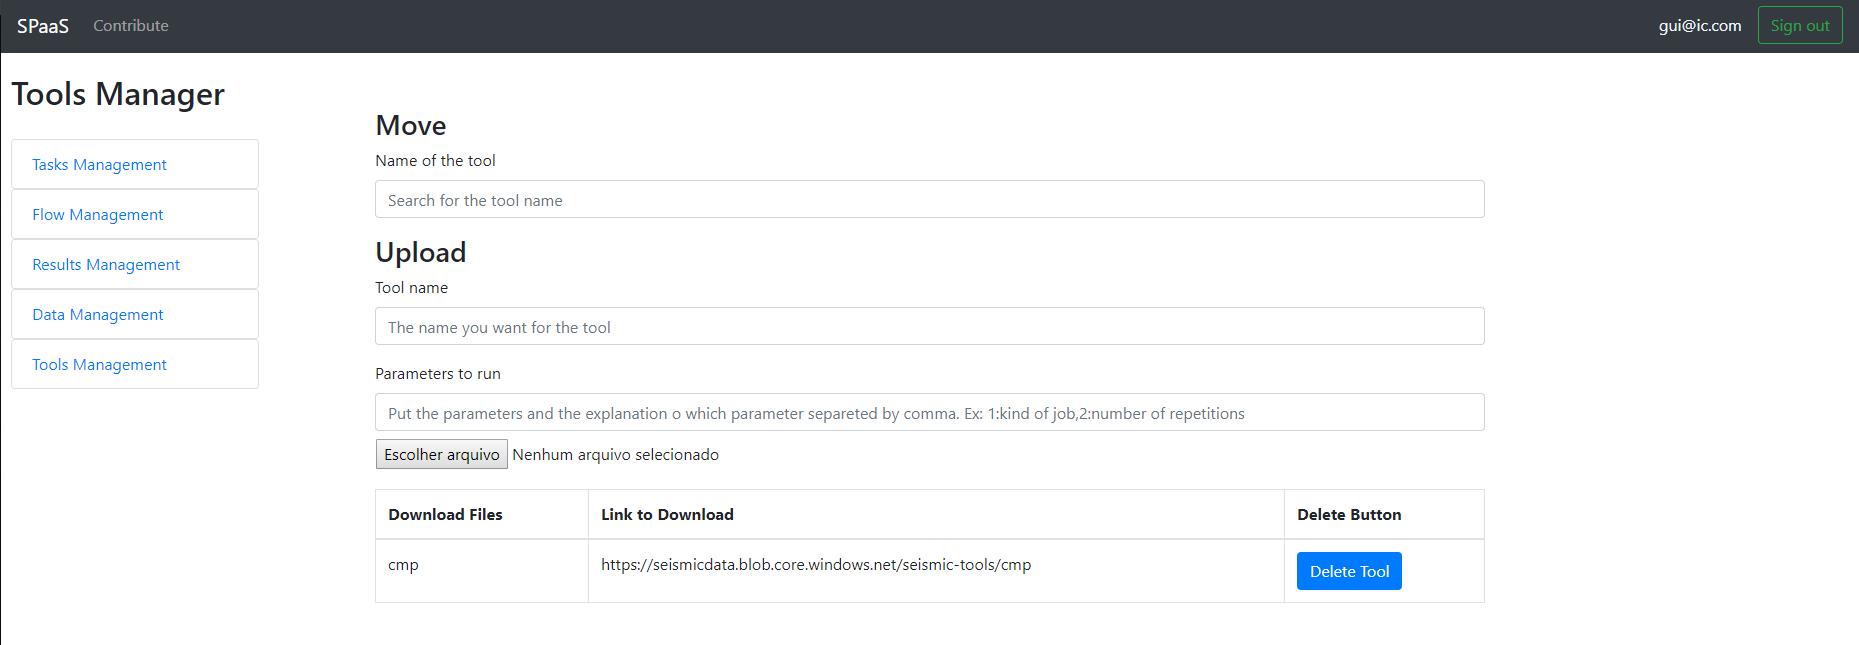
\includegraphics[scale=0.3]{tools_final.eps}
  \caption{Tela final de gerenciamento de binários}
  \label{fig:finalTools}
\end{figure}

Parecida com a tela referente aos dados, a Figura~\ref{fig:finalTools} mostra o componente de gerenciamento dos binários. Também deve
ser selecionado um arquivo, um nome e quais os parâmetros necessários para a execução, juntamente com suas explicações. Os parâmetros são submetidos da seguinte maneira: 1:explicação do parâmetro 1,
2:explicação do parâmetro 2, etc.

\begin{figure}[!h]
  \centering
  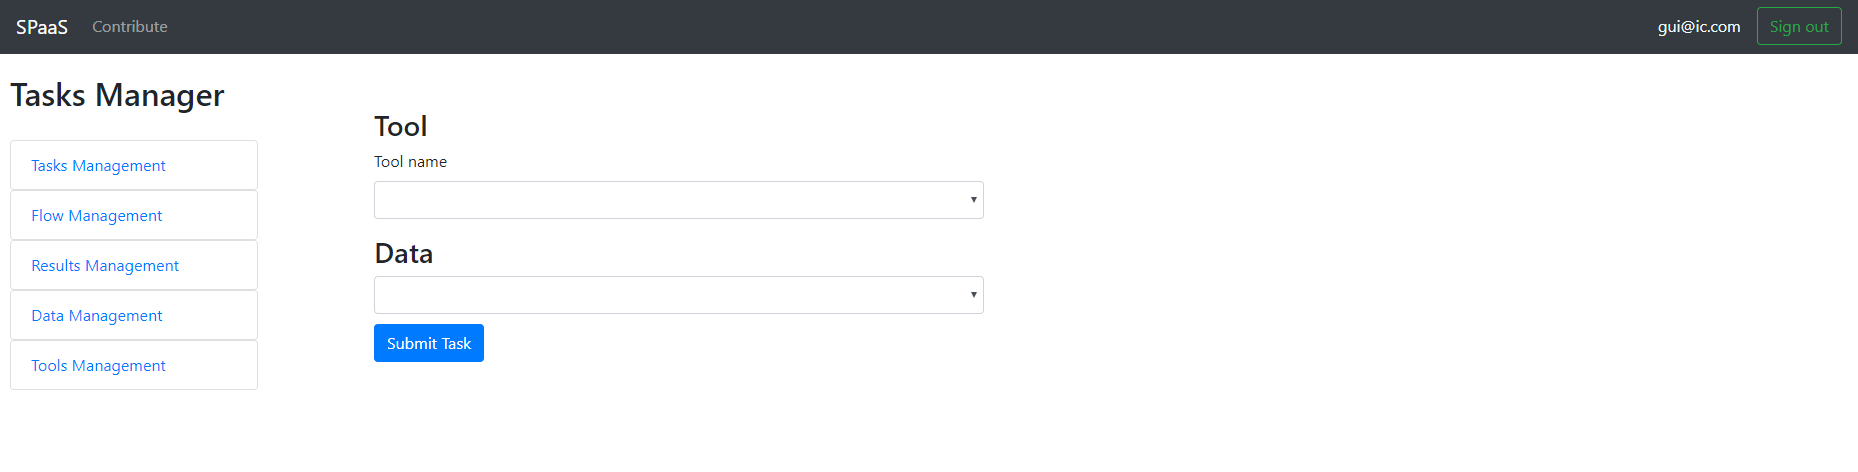
\includegraphics[scale=0.3]{task_first_final.eps}
  \caption{Tela final de gerencimento de processamentos}
  \label{fig:finalTasks}
\end{figure}

\begin{figure}[!h]
  \centering
  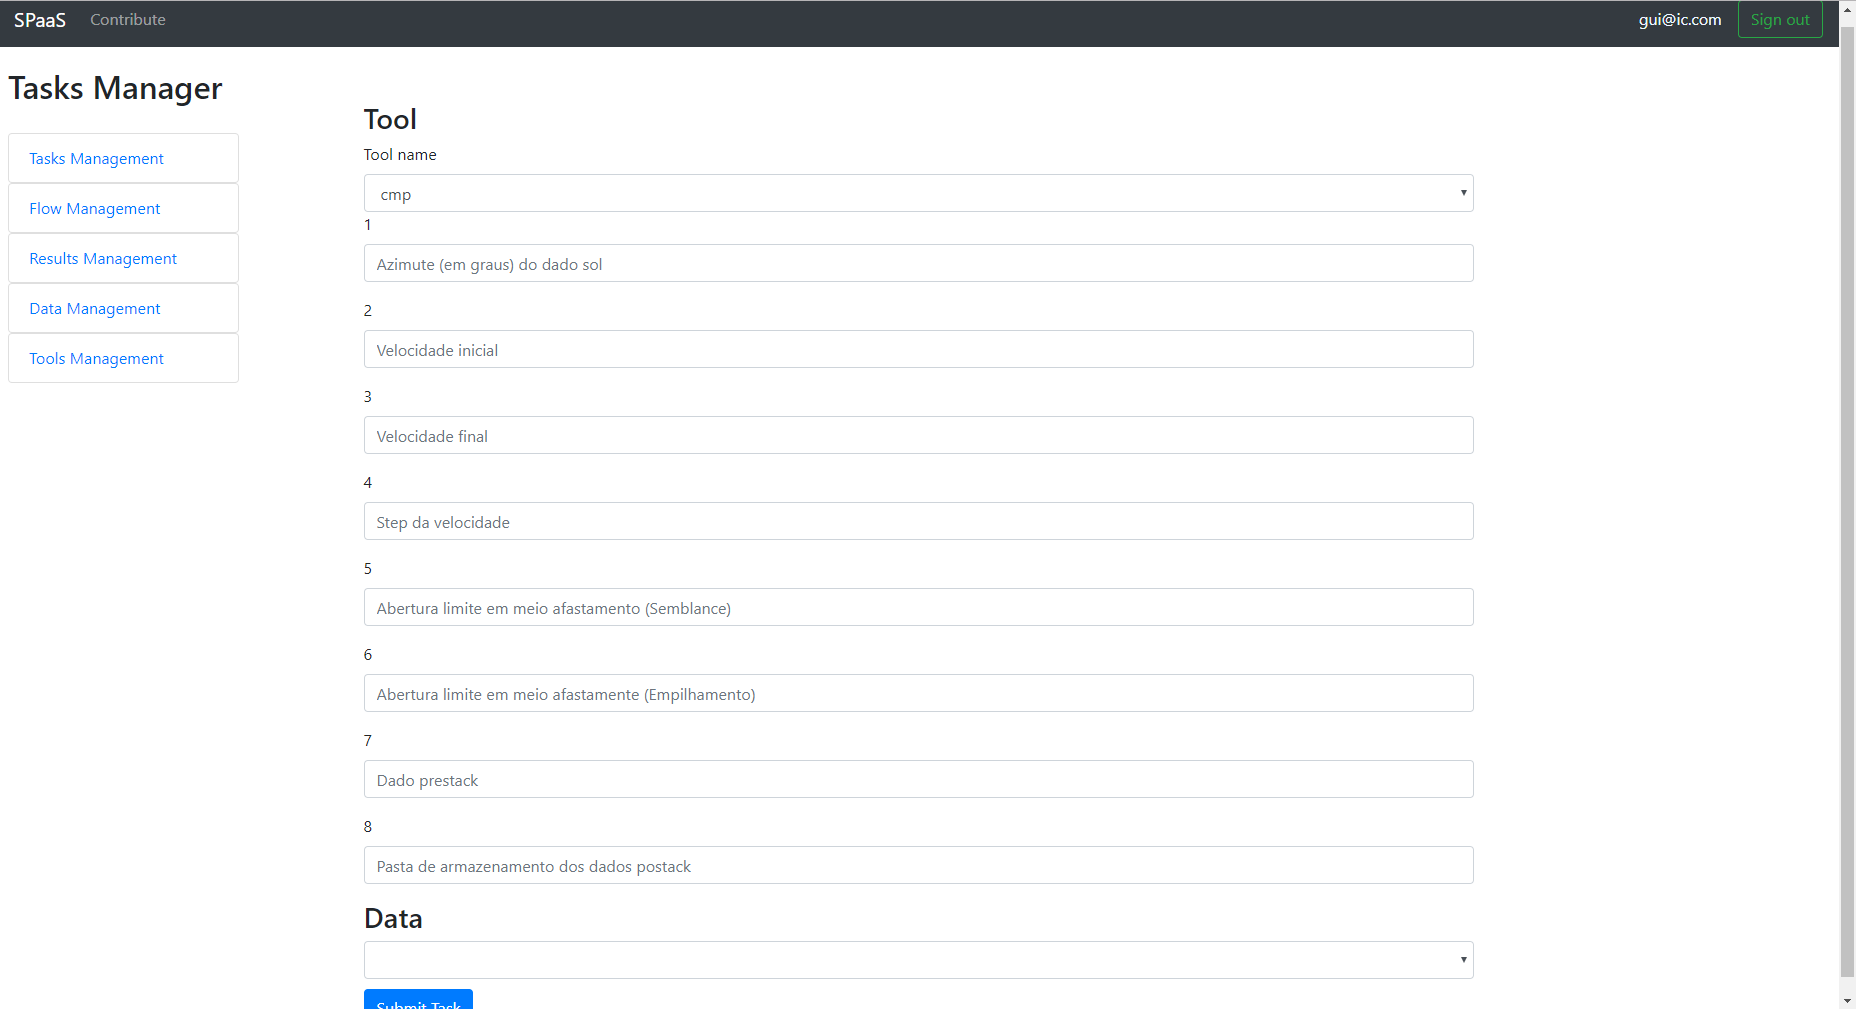
\includegraphics[scale=0.3]{task_args_final.eps}
  \caption{Tela final de processamento detalhada}
  \label{fig:finalDetailedTask}
\end{figure}

A Figura~\ref{fig:finalTasks} mostra como é a definição de um pedido de processamento. Nesse primeiro momento, só é possível escolher um binário e o dado que serão usados, porém como mostra 
a Figura~\ref{fig:finalDetailedTask}, após selecionar o binário, serão automaticamente carregados quais são os argumentes necessários para a execução dessa tarefa. Esses argumentos
foram submetidos juntamente com o binário na tela representada pela Figura~\ref{fig:finalTools}.

\begin{figure}[!h]
  \centering
  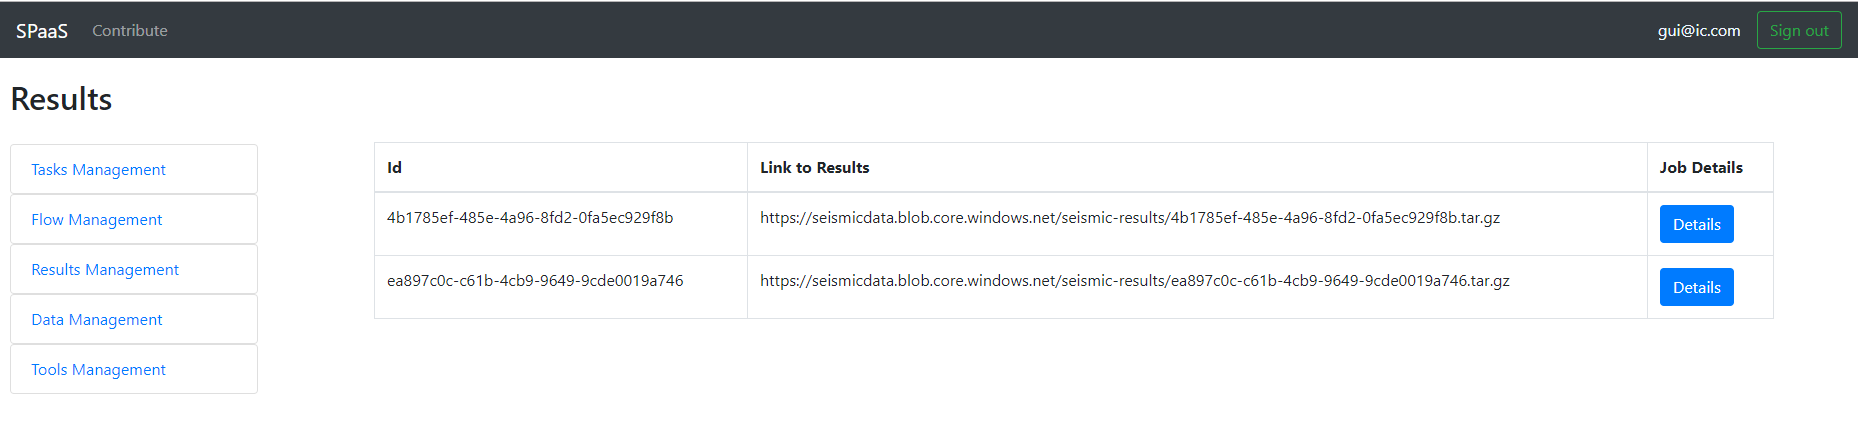
\includegraphics[scale=0.3]{results_final.eps}
  \caption{Tela final de gerenciamento de resultados}
  \label{fig:finalResults}
\end{figure}

\begin{figure}[!h]
  \centering
  
\includegraphics[scale=0.6]{results_detail_final.eps}
  \caption{Tela final com detalhes do processamento nos resultados}
  \label{fig:finalResultsDetail}
\end{figure}

Na tela de resultados, ilustrada pela Figura~\ref{fig:finalResults}, fica claro como podemos obter os resultados depois de terminados os processamentos. Além disso, caso o usuário queira verificar 
quais foram os dados, binários e argumentos que geraram aqueles resultados, é possível através do botão de \emph{details}, que gera o Json com as características daquele processamento, como é possível ver na 
Figura~\ref{fig:finalResultsDetail}.

\begin{thebibliography}{99}

\bibitem{UPP} A. Back and Hugo Lindén., {\it Cloud Computing Security: A Systematic Literature Review,} (2015).

\bibitem{HPC} K. Paladugu and S. Mukka, {\it Systematic Literature Review and Survey on High Performance Computing in Cloud,} (2012).

\bibitem{BB} B. Burns, {\it Designing Distributed Systems,} (2017).

\bibitem{BORG} A. Verma, L. Pedrosa  et al., {\it Large-scale cluster management at Google with Borg,} (2015).

\end{thebibliography}

\end{document}

